\documentclass{article}

\usepackage{amsmath}
\usepackage{amssymb}
\usepackage{amsthm}
\usepackage{amsfonts}

\usepackage{tikz}
\usepackage{color}
\usetikzlibrary{calc,shapes,fadings,automata,backgrounds,petri,shapes,decorations,decorations.pathmorphing,decorations.pathreplacing}


\newcommand{\pn}{Petri net}
\newcommand{\pns}{Petri nets}
\newcommand{\apical}{$A\pi$-calculus}
\newcommand{\pical}{$\pi$-calculus}
\newcommand{\nest}{\mathit{nest}_\nu}
\newcommand{\depth}{\mathit{depth}}
\newcommand{\set}[1]{\left\{#1\right\}}
\newcommand{\pset}[2]{\set{\,#1\mid#2\,}}
\newcommand{\process}{\mathcal{P}}
\newcommand{\Reach}{\mathit{Reach}}
\newcommand{\subgraph}{\mathrel{\hookrightarrow}}

\newcommand{\tikzMessage}[1]{
  \draw[thick,fill=white] (#1) rectangle ++(0.6, -0.4);
  \path[draw,-,thick] (#1) -- ++(0.3, -0.2) -- ++(0.3, 0.2); 
}
\newcommand{\tikzMessageNode}[2]{
  \node[draw,thick,fill=white,rectangle,inner sep=0pt,minimum height=0.4cm,minimum width=0.6cm] (#1) at (#2) {};
  \path[draw,-,thick] (#2) -- ++(-0.3, 0.2) (#2) -- ++(0.3, 0.2); 
}

\begin{document}
  
  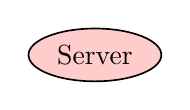
\begin{tikzpicture}[semithick, ->, node distance=2cm]
  \node [draw,ellipse,fill=red!20]  (x) at ( 0, 0) {Server};
  \end{tikzpicture}
%
  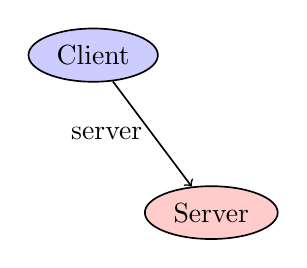
\begin{tikzpicture}[semithick, ->, node distance=2cm]
  \node [draw,ellipse,fill=red!20]  (x) at ( 0, 0) {Server};
  \node [draw,ellipse,fill=blue!20] (ni) at (-1.5, 2) {Client};
  \path  (ni) edge node [left] {server} (x);
  \end{tikzpicture}
%
  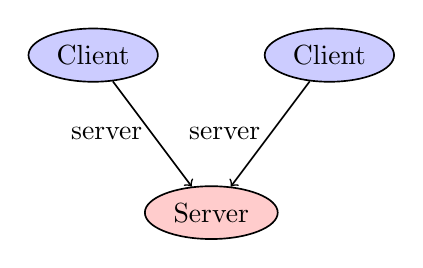
\begin{tikzpicture}[semithick, ->, node distance=2cm]
  \node [draw,ellipse,fill=red!20]  (x) at ( 0, 0) {Server};
  \node [draw,ellipse,fill=blue!20] (ni) at (-1.5, 2) {Client};
  \path  (ni) edge node [left] {server} (x);
  \node [draw,ellipse,fill=blue!20] (nj) at ( 1.5, 2) {Client};
  \path  (nj) edge node [left] {server} (x);
  \end{tikzpicture}
%
  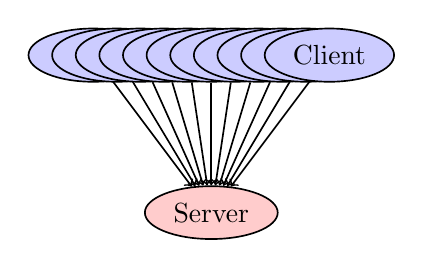
\begin{tikzpicture}[semithick, ->, node distance=2cm]
  \node [draw,ellipse,fill=red!20]  (x) at ( 0, 0) {Server};
  \node [draw,ellipse,fill=blue!20] (ni) at (-1.5, 2) {Client};
  \path  (ni) edge node [left] {} (x);
  \node [draw,ellipse,fill=blue!20] (n1) at (-1.2, 2) {Client};
  \path  (n1) edge (x);
  \node [draw,ellipse,fill=blue!20] (n2) at (-0.9, 2) {Client};
  \path  (n2) edge (x);
  \node [draw,ellipse,fill=blue!20] (n3) at (-0.6, 2) {Client};
  \path  (n3) edge (x);
  \node [draw,ellipse,fill=blue!20] (n4) at (-0.3, 2) {Client};
  \path  (n4) edge (x);
  \node [draw,ellipse,fill=blue!20] (n5) at ( 0  , 2) {Client};
  \path  (n5) edge (x);
  \node [draw,ellipse,fill=blue!20] (n6) at ( 0.3, 2) {Client};
  \path  (n6) edge (x);
  \node [draw,ellipse,fill=blue!20] (n7) at ( 0.6, 2) {Client};
  \path  (n7) edge (x);
  \node [draw,ellipse,fill=blue!20] (n8) at ( 0.9, 2) {Client};
  \path  (n8) edge (x);
  \node [draw,ellipse,fill=blue!20] (n9) at ( 1.2, 2) {Client};
  \path  (n9) edge (x);
  \node [draw,ellipse,fill=blue!20] (nj) at ( 1.5, 2) {Client};
  \path  (nj) edge (x);
  \end{tikzpicture}

  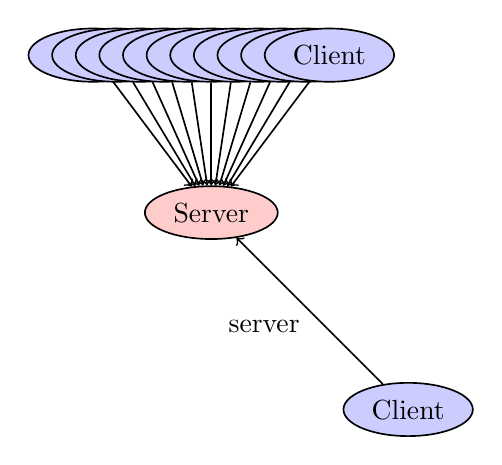
\begin{tikzpicture}[semithick, ->, node distance=2cm]
  \node [draw,ellipse,fill=red!20]  (x) at ( 0, 0) {Server};
  \node [draw,ellipse,fill=blue!20] (ni) at (-1.5, 2) {Client};
  \path  (ni) edge node [left] {} (x);
  \node [draw,ellipse,fill=blue!20] (n1) at (-1.2, 2) {Client};
  \path  (n1) edge (x);
  \node [draw,ellipse,fill=blue!20] (n2) at (-0.9, 2) {Client};
  \path  (n2) edge (x);
  \node [draw,ellipse,fill=blue!20] (n3) at (-0.6, 2) {Client};
  \path  (n3) edge (x);
  \node [draw,ellipse,fill=blue!20] (n4) at (-0.3, 2) {Client};
  \path  (n4) edge (x);
  \node [draw,ellipse,fill=blue!20] (n5) at ( 0  , 2) {Client};
  \path  (n5) edge (x);
  \node [draw,ellipse,fill=blue!20] (n6) at ( 0.3, 2) {Client};
  \path  (n6) edge (x);
  \node [draw,ellipse,fill=blue!20] (n7) at ( 0.6, 2) {Client};
  \path  (n7) edge (x);
  \node [draw,ellipse,fill=blue!20] (n8) at ( 0.9, 2) {Client};
  \path  (n8) edge (x);
  \node [draw,ellipse,fill=blue!20] (n9) at ( 1.2, 2) {Client};
  \path  (n9) edge (x);
  \node [draw,ellipse,fill=blue!20] (nj) at ( 1.5, 2) {Client};
  \path  (nj) edge (x);
  \node [draw,ellipse,fill=blue!20] (m) at ( 2.5, -2.5) {Client};
  \path  (m) edge node [below left] {server} (x);
  \end{tikzpicture}

  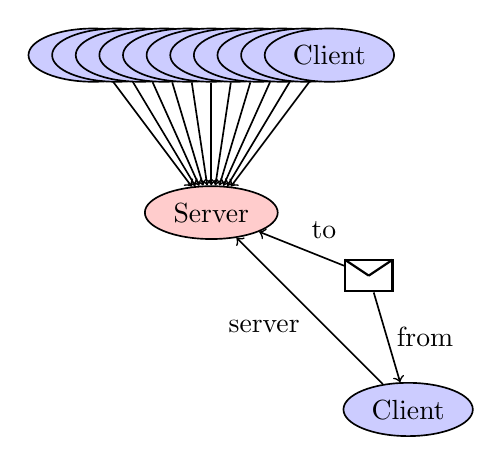
\begin{tikzpicture}[semithick, ->, node distance=2cm]
  \node [draw,ellipse,fill=red!20]  (x) at ( 0, 0) {Server};
  \node [draw,ellipse,fill=blue!20] (ni) at (-1.5, 2) {Client};
  \path  (ni) edge (x);
  \node [draw,ellipse,fill=blue!20] (n1) at (-1.2, 2) {Client};
  \path  (n1) edge (x);
  \node [draw,ellipse,fill=blue!20] (n2) at (-0.9, 2) {Client};
  \path  (n2) edge (x);
  \node [draw,ellipse,fill=blue!20] (n3) at (-0.6, 2) {Client};
  \path  (n3) edge (x);
  \node [draw,ellipse,fill=blue!20] (n4) at (-0.3, 2) {Client};
  \path  (n4) edge (x);
  \node [draw,ellipse,fill=blue!20] (n5) at ( 0  , 2) {Client};
  \path  (n5) edge (x);
  \node [draw,ellipse,fill=blue!20] (n6) at ( 0.3, 2) {Client};
  \path  (n6) edge (x);
  \node [draw,ellipse,fill=blue!20] (n7) at ( 0.6, 2) {Client};
  \path  (n7) edge (x);
  \node [draw,ellipse,fill=blue!20] (n8) at ( 0.9, 2) {Client};
  \path  (n8) edge (x);
  \node [draw,ellipse,fill=blue!20] (n9) at ( 1.2, 2) {Client};
  \path  (n9) edge (x);
  \node [draw,ellipse,fill=blue!20] (nj) at ( 1.5, 2) {Client};
  \path  (nj) edge (x);
  \node [draw,ellipse,fill=blue!20] (m) at ( 2.5, -2.5) {Client};
  \path  (m) edge node [below left] {server} (x);
  \tikzMessageNode{mm}{2.0,-0.8}
  \path  (mm) edge node [right] {from} (m);
  \path  (mm) edge node [above right] {to} (x);
  \end{tikzpicture}

  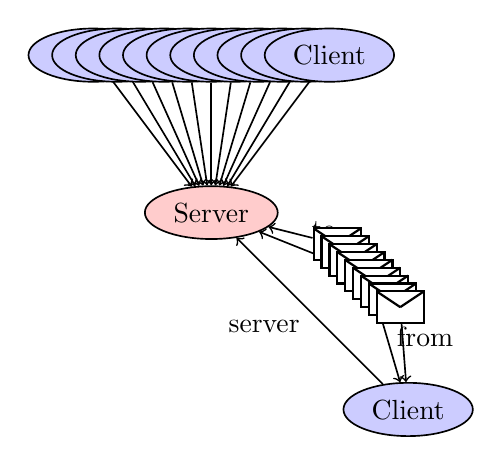
\begin{tikzpicture}[semithick, ->, node distance=2cm]
  \node [draw,ellipse,fill=red!20]  (x) at ( 0, 0) {Server};
  \node [draw,ellipse,fill=blue!20] (ni) at (-1.5, 2) {Client};
  \path  (ni) edge (x);
  \node [draw,ellipse,fill=blue!20] (n1) at (-1.2, 2) {Client};
  \path  (n1) edge (x);
  \node [draw,ellipse,fill=blue!20] (n2) at (-0.9, 2) {Client};
  \path  (n2) edge (x);
  \node [draw,ellipse,fill=blue!20] (n3) at (-0.6, 2) {Client};
  \path  (n3) edge (x);
  \node [draw,ellipse,fill=blue!20] (n4) at (-0.3, 2) {Client};
  \path  (n4) edge (x);
  \node [draw,ellipse,fill=blue!20] (n5) at ( 0  , 2) {Client};
  \path  (n5) edge (x);
  \node [draw,ellipse,fill=blue!20] (n6) at ( 0.3, 2) {Client};
  \path  (n6) edge (x);
  \node [draw,ellipse,fill=blue!20] (n7) at ( 0.6, 2) {Client};
  \path  (n7) edge (x);
  \node [draw,ellipse,fill=blue!20] (n8) at ( 0.9, 2) {Client};
  \path  (n8) edge (x);
  \node [draw,ellipse,fill=blue!20] (n9) at ( 1.2, 2) {Client};
  \path  (n9) edge (x);
  \node [draw,ellipse,fill=blue!20] (nj) at ( 1.5, 2) {Client};
  \path  (nj) edge (x);
  \node [draw,ellipse,fill=blue!20] (m) at ( 2.5, -2.5) {Client};
  \path  (m) edge node [below left] {server} (x);
  \tikzMessageNode{mm}{2.0,-0.8}
  \path  (mm) edge node [right] {from} (m);
  \path  (mm) edge node [above right] {to} (x);
  \tikzMessageNode{m1}{1.6,-0.4}
  \tikzMessageNode{m3}{1.7,-0.5}
  \tikzMessageNode{m4}{1.8,-0.6}
  \tikzMessageNode{m5}{1.9,-0.7}
  \tikzMessageNode{m6}{2.0,-0.8}
  \tikzMessageNode{m7}{2.1,-0.9}
  \tikzMessageNode{m8}{2.2,-1.0}
  \tikzMessageNode{m9}{2.3,-1.1}
  \tikzMessageNode{m2}{2.4,-1.2}
  \path  (m2) edge (m);
  \path  (m1) edge (x);
  \end{tikzpicture}
\end{document}
